\subsection{Optimización y calibración}
\label{sec:optimizacion-cal}

La resolución asignó cada renglón a un concepto (Sección~\ref{sec:algoritmo-resolucion}), y cada concepto
reúne uno o más productos candidatos. Eso no basta para entregar un kit: falta escoger un producto por
renglón, y esa elección es un compromiso entre costo, marca, disponibilidad y personaje. Este problema es
la fase de modelado (\emph{Modeling}) de CRISP-DM en la Fase~4 (OE4).  La sección lo formaliza, lo
resuelve y lo calibra; sus límites se reúnen en la Sección~\ref{sec:amenazas}. La
Figura~\ref{fig:calibracion-flujo} resume el proceso de calibración, y cada caja remite a la gráfica o a la
tabla del Anexo~\ref{anx:calibracion}, que queda como consulta.

\begin{figure}[!htb]
\centering
\resizebox{\textwidth}{!}{% Proceso de calibración del optimizador, de los datos a la evaluación en las listas de prueba.
% Misma paleta que c4-contenedores.tex. Las cifras salen de los macros \cal* de sections/cifras_calibracion.tex.

\definecolor{tkPerF}{HTML}{FFF0B8}\definecolor{tkPerB}{HTML}{9A7B00}
\definecolor{tkAppF}{HTML}{CFE2F7}\definecolor{tkAppB}{HTML}{1F4E86}
\definecolor{tkProcF}{HTML}{D3EDD0}\definecolor{tkProcB}{HTML}{2E6B2B}
\definecolor{tkExtF}{HTML}{FAD7B5}\definecolor{tkExtB}{HTML}{A8500F}
\definecolor{tkInfF}{HTML}{DEDEDE}\definecolor{tkInfB}{HTML}{4D4D4D}
\definecolor{tkBdF}{HTML}{CDEBEB}\definecolor{tkBdB}{HTML}{1C6E6E}
\definecolor{tkMqF}{HTML}{E2D6F4}\definecolor{tkMqB}{HTML}{5B2E99}
\begin{tikzpicture}[x=1cm, y=1cm, font=\scriptsize,
  per/.style={draw, thick, rounded corners=7pt, align=center, draw=tkPerB, fill=tkPerF, inner sep=3pt, minimum height=7mm},
  cont/.style={draw, rounded corners=2pt, align=center, draw=tkAppB, fill=tkAppF, inner sep=2pt, minimum height=8mm},
  proc/.style={draw, rounded corners=2pt, align=center, draw=tkProcB, fill=tkProcF, inner sep=2pt, minimum height=7mm},
  ext/.style={draw, rounded corners=2pt, align=center, draw=tkExtB, fill=tkExtF, inner sep=2pt, minimum height=7mm},
  infra/.style={draw, rounded corners=2pt, align=center, draw=tkInfB, fill=tkInfF, inner sep=2pt, minimum height=7mm},
  bd/.style={draw, cylinder, shape border rotate=90, aspect=0.22, align=center, fill=tkBdF,
    minimum width=1.25cm, draw=tkBdB, minimum height=8mm, inner sep=1pt},
  grupo/.style={draw=black!55, rounded corners=3pt, fill=black!4},
  http/.style={-{Stealth[length=1.6mm]}, semithick},
  evt/.style={-{Stealth[length=1.6mm]}, densely dashed, semithick},
  cola/.style={-{Stealth[length=1.6mm]}, semithick, draw=tkMqB},
  hueco/.style={draw=white, line width=2.8pt},
  paso/.style={circle, draw, fill=white, inner sep=0.5pt, font=\scriptsize\bfseries, minimum size=4.4mm},
  rot/.style={font=\scriptsize, fill=white, inner sep=1pt},
  etapa/.style={draw, thick, rounded corners=3pt, align=left, inner sep=4pt, text width=4.7cm, minimum height=3.1cm, anchor=north west},
  tit/.style={font=\footnotesize\bfseries, anchor=north west, inner sep=0pt},
  ref/.style={font=\scriptsize\itshape, anchor=south west, inner sep=0pt}]
\def\caja#1#2#3#4#5#6{% color, posición, título, cuerpo, dónde se ve, nombre
  \node[etapa, draw=tk#1B, fill=tk#1F] (#6) at #2 {};
  \node[tit] at ([shift={(4pt,-4pt)}]#6.north west) {#3};
  \node[anchor=north west, text width=4.4cm, align=left, inner sep=0pt] at ([shift={(4pt,-0.75cm)}]#6.north west) {#4};
  \node[ref] at ([shift={(4pt,4pt)}]#6.south west) {#5};}
\caja{Bd}{(0,0)}{1. Datos y pliegues}{\calListas{} listas de \calColegios{} colegios.\\
  Prueba: \calColegiosPrueba{} colegios, \calHVListas{} listas, apartadas antes de mirar resultados.\\
  Ajuste: \calPliegues{} pliegues por colegio, \calCVListas{} listas.}{Tabla~\ref{tab:calopt-rejilla}}{p1}
\caja{App}{(5.7,0)}{2. Umbral: exacto o NSGA-II}{\calSubproblemas{} subproblemas medidos.\\
  Ajuste del exacto: $t\approx\calConstante\,S^{\calExponente}$ s.\\
  Cruce de los dos métodos y umbral $\Lambda=\calLimite$.}{Fig.~\ref{fig:calibracion-graficas}a, Tab.~\ref{tab:calopt-umbral}}{p2}
\caja{App}{(11.4,0)}{3. Rejilla $a$, $b$}{$a,b\in\{\calFactores\}$.\\
  Se elige la configuración más barata a menos de \calUmbralHV{} del mejor hipervolumen.\\
  Elegida: $a=b=\calA$.}{Fig.~\ref{fig:calibracion-graficas}b, Tab.~\ref{tab:calopt-rejilla}}{p3}
\caja{Mq}{(0,-4.3)}{4. Pesos MAUT desde la P21}{\calEncuestados{} acudientes ordenan cuatro criterios.\\
  Precio \calWPrecio, marca \calWMarca, calidad \calWCalidad, personaje \calWPersonaje.\\
  IC 95\,\% por \emph{bootstrap}.}{Fig.~\ref{fig:calibracion-graficas}c}{p4}
\caja{Mq}{(5.7,-4.3)}{5. Sensibilidad Dirichlet}{\calSensListas{} listas y \calSensPerturbaciones{} sorteos de pesos dentro de los intervalos.\\
  El kit recomendado se mantiene en al menos \calSensICMin{} de los sorteos.}{Fig.~\ref{fig:calibracion-graficas}d, Tab.~\ref{tab:calopt-sensibilidad}}{p5}
\caja{Proc}{(11.4,-4.3)}{6. Umbral de similitud $\tau$}{$\tau=0{,}75$ se evalúa y se conserva.\\
  \calTauPares{} pares de \calTauColegios{} colegios; AUC \calTauAUC, precisión \calTauPrecision.}{Fig.~\ref{fig:tau-clasificacion}, Sec.~\ref{sec:recuperacion}}{p6}
\caja{Ext}{(0,-8.6)}{7. Evaluación en prueba}{Hipervolumen relativo al frente exacto: \calHVFrente{} en las \calHVListas{} listas; \calPruebaElegidaHV{} en las \calHVListasNsga{} con NSGA-II.\\
  Un solo kit cubre menos: MAUT \calHVMAUTPesos, Ahorrador \calHVAhorrador, Premium \calHVPremium.}{Fig.~\ref{fig:calibracion-graficas}e, Tab.~\ref{tab:calopt-hv}}{p7}
% Flechas del proceso
\draw[http] (p1.east |- 0,-1.5) -- (p2.west |- 0,-1.5);
\draw[http] (p2.east |- 0,-1.5) -- (p3.west |- 0,-1.5);
\draw[http] (p3.south) -- ++(0,-0.55) -| node[rot, pos=0.25] {configuración elegida} (p4.north);
\draw[http] (p4.east |- 0,-5.8) -- (p5.west |- 0,-5.8);
\draw[http] (p5.east |- 0,-5.8) -- (p6.west |- 0,-5.8);
\draw[http] (p6.south) -- ++(0,-0.55) -| node[rot, pos=0.25] {pesos y $\tau$ fijados} (p7.north);
% Leyenda
\def\tkley#1#2#3#4{\node[#1, minimum width=7mm, minimum height=4.2mm, inner sep=0pt, text width=7mm] at #2 {};
  \node[anchor=west, font=\scriptsize, inner sep=1pt] at ([xshift=4.5mm]#2) {#3};}
\node[draw=black!40, rounded corners=2pt, anchor=north west, minimum width=10.2cm, minimum height=1.9cm,
  inner sep=0pt] (cajaley) at (6.2,-8.6) {};
\node[anchor=north west, font=\scriptsize\bfseries] at ([shift={(2mm,-1mm)}]cajaley.north west) {Leyenda};
\begin{scope}[shift={(cajaley.north west)}]
\node[draw=tkBdB, fill=tkBdF, rounded corners=2pt, minimum width=7mm, minimum height=4.2mm] at (0.9,-0.75) {};
\node[anchor=west, font=\scriptsize] at (1.4,-0.75) {Datos};
\node[draw=tkAppB, fill=tkAppF, rounded corners=2pt, minimum width=7mm, minimum height=4.2mm] at (3.2,-0.75) {};
\node[anchor=west, font=\scriptsize] at (3.7,-0.75) {Optimizador};
\node[draw=tkMqB, fill=tkMqF, rounded corners=2pt, minimum width=7mm, minimum height=4.2mm] at (6.2,-0.75) {};
\node[anchor=west, font=\scriptsize] at (6.7,-0.75) {Pesos MAUT};
\node[draw=tkProcB, fill=tkProcF, rounded corners=2pt, minimum width=7mm, minimum height=4.2mm] at (0.9,-1.4) {};
\node[anchor=west, font=\scriptsize] at (1.4,-1.4) {Umbral $\tau$};
\node[draw=tkExtB, fill=tkExtF, rounded corners=2pt, minimum width=7mm, minimum height=4.2mm] at (3.2,-1.4) {};
\node[anchor=west, font=\scriptsize] at (3.7,-1.4) {Evaluación};
\draw[http] (6.0,-1.4) -- +(0.7,0); \node[anchor=west, font=\scriptsize] at (6.8,-1.4) {Paso siguiente};
\end{scope}
\end{tikzpicture}
}
\caption[Proceso de calibración del optimizador.]{Proceso de calibración del optimizador, de los
datos a la evaluación en las listas de prueba. Cada caja trae su cifra principal y la figura o tabla
donde se ve.}
\label{fig:calibracion-flujo}
\end{figure}

\paragraph{Análisis del problema.} Cada producto que satisface un renglón comprable se llama \emph{candidato}. Sea $n$ el número de
\emph{líneas decidibles}, es decir, los renglones con al menos un candidato admisible, y sea $C_i$
el conjunto de candidatos de la línea $i$. Un kit es una asignación
$\mathbf{x}=(x_1,\dots,x_n)$ con $x_i\in C_i$, y el espacio de búsqueda tiene
$S=\prod_{i=1}^{n}|C_i|$ asignaciones, de modo que crece de forma exponencial con las líneas:
basta con dos candidatos por línea para que $S\geq 2^n$. Cada kit se evalúa con cuatro objetivos
($M=4$): el costo $f_1$, que se minimiza, y la fidelidad de marca $f_2$, la disponibilidad $f_3$ y
el personaje $f_4$, normalizados en $[0,1]$, que se maximizan. Como el candidato más barato rara
vez es el de mejor marca, no existe en general un kit que sea el mejor en los cuatro. Por eso se
busca el \emph{frente de Pareto} $\mathcal{P}$, el conjunto de kits que ningún otro domina, donde
un kit domina a otro si no es peor en ningún objetivo y es mejor en al menos uno. Como el acudiente compra un solo kit, sobre $\mathcal{P}$ hay que escoger un
punto según sus preferencias. Las \calListas{} instancias del banco salen de 174 listas de
\calColegios{} colegios: \calListasNsga{} superan el umbral de enumeración, \calListasExacto{} quedan
por debajo, y el espacio más grande es del orden de $10^{\calEspacioMaxLog}$.

\paragraph{Modelo formal.} Para fijar el problema se usan variables de decisión binarias. Sea
$x_{i,p}\in\{0,1\}$ igual a 1 si se elige el producto $p$ para la línea decidible $i$, con
$\sum_{p\in C_i}x_{i,p}=1$ para cada $i$, de modo que cada línea recibe exactamente un producto. El código usa una forma equivalente: la variable de la línea $i$ es el índice entero del candidato,
en $\{0,\dots,|C_i|-1\}$, que es la que recibe NSGA-II. Las restricciones duras son
tres y actúan en momentos distintos.
\begin{enumerate}[label=\textbf{R\arabic*.},leftmargin=*,itemsep=1pt,topsep=2pt]
\item \emph{Filtros del acudiente, antes del frente} (\texttt{aplicar\_filtros\_duros}). Si
el acudiente excluye una marca, se retira de $C_i$ todo candidato de esa marca, salvo que el colegio la
exija en el renglón; si pide solo productos disponibles, se retiran los
candidatos sin oferta vigente. Si $C_i$ queda vacío, la línea pasa a ser un hueco del catálogo con un
mensaje. Se hace antes porque una restricción dura no debe
competir como un peso más.
\item \emph{Admisibilidad} (\texttt{\_admisibles}). Una línea es decidible si no es informativa y
tiene candidatos. Entre ellos se prefieren los que cumplen el atributo exigido por el colegio; si
ninguno lo cumple, entran todos.
\item \emph{Tope de gasto y sobreprecio, después del frente} (\texttt{\_tope},
\texttt{elegir\_recomendado\_maut}). El tope $B$ es el presupuesto declarado, sin estirarlo con el
sobreprecio, y se exige $f_1(\mathbf{x})\leq B$ y $f_1(\mathbf{x})\leq(1+\sigma)\,c_{\min}$, con $\sigma$ el
sobreprecio aceptado y $c_{\min}$ el menor costo entre los kits del frente con la máxima disponibilidad $f_3$,
filtro que se aplica antes para recomendar solo lo que está disponible hoy. Se aplican
sobre el frente completo, porque recortarlo antes escondería opciones que el acudiente aún puede querer ver.
\end{enumerate}
La cantidad por empaque entra en el costo. Si la línea pide $q_i$ unidades y el producto $p$ trae $e_p$
unidades por empaque, se compran $u_{i,p}=\lceil q_i/e_p\rceil$ empaques (\texttt{unidades\_a\_comprar}),
que es cero si $q_i\leq 0$. Con $\pi_p$ el precio del empaque, $\rho_p\in\{0,1,2\}$ el nivel de marca
(económico, confiable, premium), $\kappa_p=1$ si el producto trae el personaje buscado y $d_p=1$ si
tiene precio, los cuatro objetivos de $\mathbf{x}$ son
\begin{align}
f_1(\mathbf{x})&=\sum_{i}\sum_{p\in C_i:\,d_p=1}x_{i,p}\,\pi_p\,u_{i,p}, &
f_2(\mathbf{x})&=\frac{1}{2n}\sum_{i}\sum_{p}x_{i,p}\,\rho_p,\label{eq:f1f2}\\
f_3(\mathbf{x})&=\frac{1}{n}\sum_{i}\sum_{p}x_{i,p}\,d_p, &
f_4(\mathbf{x})&=\frac{1}{n}\sum_{i}\sum_{p}x_{i,p}\,\kappa_p.\label{eq:f3f4}
\end{align}
El costo $f_1$ está en pesos y suma solo los productos con precio, de modo que la
falta de precio baja $f_3$ y no abarata el kit. Los otros tres son promedios por línea en $[0,1]$:
$f_2$ divide el nivel de marca entre su máximo, 2; $f_3$ es la fracción de líneas
disponibles hoy; y $f_4$ es la fracción de líneas con el personaje pedido, o con cualquiera
si no se pidió ninguno. El problema es entonces minimizar
$(f_1,-f_2,-f_3,-f_4)$ sobre las asignaciones que cumplen R1 y R2; R3 se aplica al escoger el punto.

\paragraph{Diseño: entradas y salidas.} La Tabla~\ref{tab:es-optimizador} define los tipos.

\begin{table}[H]
\centering\footnotesize
\caption{Entradas y salidas del optimizador del kit.}
\label{tab:es-optimizador}
\begin{tabularx}{\textwidth}{@{}p{2.6cm}p{4.4cm}X@{}}
\toprule
Elemento & Tipo & Descripción \\
\midrule
Entrada $C_1,\dots,C_n$ & conjuntos no vacíos de candidatos & Cada candidato trae precio en pesos (o ninguno), unidades por empaque, nivel de marca en $\{0,1,2\}$ y personaje; cada línea trae su cantidad \\
Entrada $\mathbf{w}$ & cuatro reales no negativos & Pesos de precio, marca exigida, calidad y personaje; por omisión, los de la encuesta \\
Entradas $B$ y $\sigma$ & entero positivo y real en $[0,1]$, opcionales & Tope de gasto por hijo y sobreprecio aceptado sobre el kit más barato \\
Parámetros & entero $\Lambda$ y semilla $s$ & Umbral de enumeración y semilla del generador, para que el frente sea reproducible \\
Salida $\mathcal{P}$ & kits no dominados con su vector $(f_1,\dots,f_4)$ & Exacto si $S\leq\Lambda$ y aproximado si $S>\Lambda$, ordenado por costo \\
Salida $\mathbf{x}^\star$ & kit de $\mathcal{P}$ o nulo & Kit recomendado; nulo si ninguno cumple el tope y el sobreprecio \\
\bottomrule
\end{tabularx}
\end{table}

\paragraph{Estrategia algorítmica.} La estrategia tiene dos fases: primero se calcula el frente y
después se escoge un punto sobre él. Para la primera fase, el tamaño del espacio decide el método.
Si $S\leq\Lambda$, se enumeran las $S$ asignaciones y se conservan las no dominadas, lo que da el
frente exacto sin depender de ninguna semilla. Si $S>\Lambda$, se corre NSGA-II
\citep{deb_fast_2002} sobre pymoo \citep{blank_pymoo_2020}, un algoritmo evolutivo que mantiene una
\emph{población} de $N$ kits y, en cada una de las $G$ \emph{generaciones}, produce descendientes
por cruce y mutación y conserva los mejores. La población inicial se siembra con los kits que arma una regla sencilla para cada perfil, de modo que
el frente aproximado nunca queda por debajo de ellos. El algoritmo conserva los mejores kits según su
rango de dominancia y, entre los de igual rango, los más alejados de sus vecinos (la distancia de
apiñamiento), para que el frente no se concentre en una sola zona. La corrida termina tras un número
fijo de generaciones para que la misma semilla reproduzca el mismo frente.

La segunda fase usa la teoría de la utilidad multiatributo (MAUT) \citep{keeney_decisions_1976}
\emph{a posteriori}, es decir, primero se calcula el frente y después las preferencias escogen sobre
él \citep{miettinen_nonlinear_1999}. Para cada objetivo se define una utilidad $u_j$, lineal entre
el peor y el mejor valor que alcanza el frente, y la utilidad del kit es
$U=\hat w_{\mathrm{precio}}\,u_1+(\hat w_{\mathrm{marca}}+\hat w_{\mathrm{calidad}})\,u_2+\hat w_{\mathrm{personaje}}\,u_4$,
donde $\hat{\mathbf{w}}$ son los pesos renormalizados para que sumen 1. No entra $u_3$, porque la
disponibilidad ya se fijó en su máximo. La marca exigida y la
calidad pesan sobre la misma utilidad porque el frente mide ambas con el nivel de marca. La forma
aditiva supone \emph{independencia preferencial}, es decir, que la preferencia entre dos valores de
un criterio no depende de los valores de los demás, y ese supuesto se declara. En el código, esta
fase es la función \texttt{elegir\_recomendado\_maut}, y la regla de recomendación la usa para
decidir el Premium: lo marca cuando el acudiente acepta al menos un 10\,\% de sobreprecio y MAUT lo
prefiere al Ahorrador. El Algoritmo~\ref{alg:frente-maut} reúne las dos fases.

Fuera del frente, el kit Fan se arma con una regla de presentación que se aplica después de
calcularlo. Para cada hijo y concepto, el producto de personaje va una vez en la línea donde mejor
encaja sin contradecir sus atributos exigidos, y solo se repite donde la línea pide surtido. Su costo
es $O(n\cdot a)$, con $a$ el número de atributos exigidos por línea.

\begin{algorithm}[H]
\caption{Construcción del frente y selección del kit recomendado}
\label{alg:frente-maut}
\KwEntrada{candidatos $C_1,\dots,C_n$; pesos $\mathbf{w}$; tope $B$; sobreprecio $\sigma$; umbral $\Lambda$; semilla $s$}
\KwSalida{frente $\mathcal{P}$ y kit recomendado $\mathbf{x}^\star$ (o nulo)}
$S \leftarrow \prod_{i=1}^{n}|C_i|$\;
\uIf{$S\leq 1$}{\Return{(vacío, nulo)} \tcp*{no hay decisión que tomar}}
\uElseIf{$S\leq\Lambda$}{$\mathcal{P}\leftarrow$ no dominados de $\{\mathbf{F}(\mathbf{x}) : \mathbf{x}\in C_1\times\cdots\times C_n\}$ \tcp*{exhaustivo}}
\Else{
  $N\leftarrow\mathrm{par}(\min(100,\max(20,6n)))$;\quad $G\leftarrow\min(60,\max(15,10\log_{10}S))$\;
  $Q_0\leftarrow$ kits heurísticos por perfil, completados al azar con la semilla $s$ hasta $N$\;
  \For{$g = 1,\dots,G$}{
    $R\leftarrow Q_{g-1}\cup{}$ CruceYMutación$(Q_{g-1})$\;
    $Q_g\leftarrow$ los $N$ mejores de $R$ por frente no dominado y apiñamiento\;
  }
  $\mathcal{P}\leftarrow$ no dominados de $Q_G\cup Q_0$\;
}
$D\leftarrow$ kits de $\mathcal{P}$ con la máxima disponibilidad $f_3$ \tcp*{solo lo disponible}
$c_{\min}\leftarrow$ menor costo $f_1$ en $D$\;
$K\leftarrow\{\mathbf{x}\in D : f_1(\mathbf{x})\leq B,\ f_1(\mathbf{x})\leq(1+\sigma)\,c_{\min}\}$\;
\lIf{$K$ es vacío}{\Return{$(\mathcal{P}$, nulo$)$}}
\Return{$(\mathcal{P},\ \arg\max_{\mathbf{x}\in K}U(\mathbf{x}))$} \tcp*{empates: menor costo}
\end{algorithm}

\paragraph{Complejidad y comparación con el método exhaustivo.} El exhaustivo visita las $S$
asignaciones y evalúa en cada una $M$ objetivos, con un costo de $\Theta(S\cdot M)$ evaluaciones, y
luego filtra los $V\leq S$ vectores distintos comparándolos por pares, con un costo de $O(V^2M)$ en
el peor caso; su tiempo crece, por tanto, con el tamaño del espacio. NSGA-II, en cambio, ordena en
cada generación $2N$ individuos con un costo de $O(MN^2)$ \citep{deb_fast_2002}, así que su
total es $O(G\cdot M\cdot N^2)$, que no crece con $S$ más que por $G$; a cambio, el frente que devuelve es una
aproximación. MAUT recorre el frente un número constante de veces, con un costo de
$O(|\mathcal{P}|\,M)$, despreciable frente a la construcción del frente.

En esta comparación se omite el factor $n$ de
evaluar un kit, común a los dos métodos, y $G$ y $N$ crecen con $\log S$ y $n$. Para saber desde qué tamaño conviene NSGA-II se igualan los dos costos, con la población y las
generaciones típicas cerca del umbral ($n=\calNTipico$, $N=\calPobTipica$ y $G=\calGenTipica$). Si
domina el filtro en su peor caso, con $V=S$, la igualdad $S^2M=GMN^2$ da $S=N\sqrt{G}=252\approx
2^{\calSTeoricoLog}$. Si domina la evaluación, $SM=GMN^2$ da $S=GN^2=63.504\approx 2^{\calSCuadradoLog}$.
El cruce queda entre esos dos valores, y como las constantes de cada operación difieren, el umbral
se fijó con la medición.

Para medirlo se armaron \calSubproblemas{} subproblemas con líneas reales y espacios entre $2^{\calNivelMin}$
y $2^{\calNivelMax}$, y en cada uno se midió el tiempo de pared de los dos métodos. Un
ajuste por mínimos cuadrados en escala logarítmica sobre los \calSubproblemasExacto{} enumerados da $t_{\mathrm{exh}}(S)\approx\calConstante\cdot S^{\calExponente}$~s; el exponente es
mayor que 1 porque el filtro de no dominados crece más rápido que la evaluación. NSGA-II, con la
configuración elegida, tardó una mediana de \calTNsgaElegidaMediana~s, y el ajuste la alcanza en
$S\approx\calCruceElegida$, o en $S\approx\calCruceElegidaP$ si se toma el percentil 95 del ajuste.
Por eso se fijó $\Lambda=\calLimite=2^{\calLimiteLog}$, con los factores $a$ y $b$ de población y generaciones ya elegidos sobre las mismas
instancias (párrafo \emph{Calibración de las constantes}), entre los dos cruces y dentro del rango que
predice la teoría. Por debajo del umbral, la enumeración fue más rápida en
\calExactoGanaBajoElegida{} subproblemas y, por encima, solo en \calExactoGanaSobreElegida. La
diferencia de calidad es pequeña: sobre \calCorridasHV{} corridas, la razón de
\emph{hipervolumen}, el volumen del espacio de objetivos que domina un frente hasta un punto de
referencia \citep{zitzler_multiobjective_1999}, entre el frente de NSGA-II y el exacto tuvo mediana
\calRazonHVMediana{} y mínimo \calRazonHVMin, con los cuatro ejes normalizados en $[0,1]$ y la
referencia en 1,1.  El exhaustivo pasa de dos minutos cerca de $2^{\calNivelMaxExacto}$.

\paragraph{Calibración de las constantes.} Los experimentos corrieron con semillas fijas en un \calCPU{} de
\calNucleos{} núcleos con \calRAM~GiB de memoria, Python \calPython{} y pymoo \calPymoo. Los pesos por omisión salen de la pregunta P21 de la encuesta, que pide ordenar los cuatro
criterios: el primero recibe 4 puntos y el último 1, y el peso es el puntaje medio dividido entre 10.
Con \calEncuestados{} respuestas, y con intervalos del 95\,\% por \emph{bootstrap}
\citep{efron_bootstrap_1979} (un remuestreo de las mismas respuestas que mide cuánto cambiaría el peso
con otra muestra), los pesos son precio \calWPrecio{} [\calWPrecioBajo; \calWPrecioAlto],
marca exigida \calWMarca{} [\calWMarcaBajo; \calWMarcaAlto], calidad \calWCalidad{}
[\calWCalidadBajo; \calWCalidadAlto] y personaje \calWPersonaje{} [\calWPersonajeBajo;
\calWPersonajeAlto]. Como los tres primeros intervalos se solapan, la encuesta no permite ordenar precio, marca y
calidad entre sí, y solo el personaje queda claramente por debajo (Figura~\ref{fig:calibracion-graficas}c).

Las fórmulas de partida de la población y de las generaciones eran
\[N=\min(200,\max(40,12n)),\qquad G=\min(120,\max(30,20\log_{10}S)).\] La calibración multiplicó la primera por $a$ y la segunda por
$b$, con $a,b\in\{\calFactores\}$, y escogió la configuración más barata cuyo hipervolumen medio no
bajara más de \calUmbralHV{} del mejor de la rejilla. Los datos se partieron por colegio, porque dos grados
de un mismo colegio comparten productos y marcas, y mezclarlos entre ajuste y prueba inflaría el
resultado. Antes de mirar ningún resultado se apartaron \calColegiosPrueba{} colegios como prueba, con
\calHVListas{} listas, \calPrueba{} de ellas por encima del umbral de enumeración, que son las únicas que
miden a NSGA-II. Con el resto se hizo validación cruzada en \calPliegues{} pliegues, es decir,
\calPliegues{} grupos de colegios que se dejan fuera por turnos. El hipervolumen relativo es el del
frente de cada configuración dividido entre el del mejor frente de la rejilla de $(a,b)$. La regla eligió $a=b=\calA$,
que da en producción las fórmulas del Algoritmo~\ref{alg:frente-maut}, y al dejar fuera cada pliegue
eligió lo mismo en \calPlieguesIguales. En el conjunto de prueba, usado una sola vez, la elegida
obtuvo un hipervolumen relativo medio de \calPruebaElegidaHV{} contra \calPruebaActualHV{} de la de
partida, una diferencia de \calDifHV{} con intervalo [\calDifHVBajo; \calDifHVAlto]
y $p<0{,}001$ en la prueba de rangos con signo de Wilcoxon \citep{wilcoxon_individual_1945}. En la
peor lista la elegida llegó a \calPruebaElegidaHVMin{} contra \calPruebaActualHVMin{}. La
pérdida es pequeña, y el tiempo medio por lista bajó de \calPruebaActualT~s a \calPruebaElegidaT~s.

El umbral de similitud $\tau=0{,}75$ de la resolución se evaluó y se mantuvo en su valor por omisión,
porque la única fuente humana es un solo revisor y la validación cruzada agrupada, que sugiere un
$\tau$ entre \calTauCVMin{} y \calTauCVMax{}, tiene una muestra demasiado concentrada para moverlo
(Sección~\ref{sec:recuperacion}). Para ver cuánto depende la recomendación de los pesos, se sortearon dentro de sus intervalos de la
P21. El kit recomendado se mantuvo en el 96,5\,\%, el 98,6\,\% y el 94,6\,\% de los sorteos con
sobreprecios de 5, 10 y 20\,\%, y en la peor lista, con 20\,\%, bajó al 54\,\%.

Por último, en las \calHVListas{} listas de los colegios de prueba el frente de producción alcanzó
\calHVFrente{} del hipervolumen exacto, y \calPruebaElegidaHV{} en las \calHVListasNsga{} con NSGA-II
(en las otras ocho el frente es exacto). La Figura~\ref{fig:calibracion-graficas} muestra qué se vio y qué se
decidió. En (a) el tiempo de la enumeración exacta sube en línea recta en escala logarítmica y el de
NSGA-II se mantiene cerca de un segundo; las curvas se cruzan cerca de la línea punteada, y de ahí
salió $\Lambda$, mientras la razón de hipervolumen queda en 1 casi siempre. En (b), la estrella cumple
el piso de \calUmbralHV{} con la cuarta parte de las evaluaciones del rombo de partida, y por eso se
eligió. En (c), el personaje queda aparte y los otros tres pesos se solapan. En (d), la fracción de
sorteos con el mismo kit cae con la perturbación y con el sobreprecio, pero se mantiene sobre 0,7, así
que la recomendación es estable. En (e), un solo kit cubre una fracción menor del hipervolumen exacto
(\calHVMAUTPesos{} el elegido por MAUT, \calHVAhorrador{} el Ahorrador y \calHVPremium{} el Premium),
y por eso se entrega el frente completo.

\begin{figure}[p]
\centering
{\footnotesize\textbf{(a)}}\\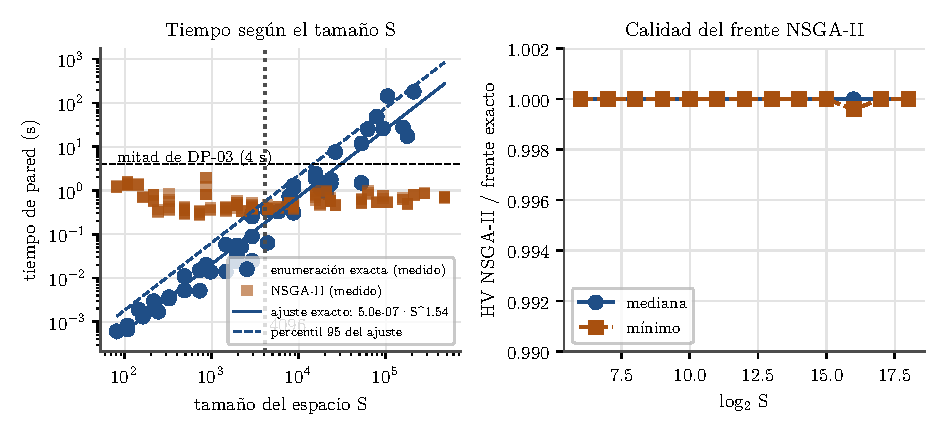
\includegraphics[width=0.82\linewidth]{img/calibracion/umbral.pdf}\\[1mm]
\begin{minipage}[t]{0.44\linewidth}\centering
{\footnotesize\textbf{(b)}}\\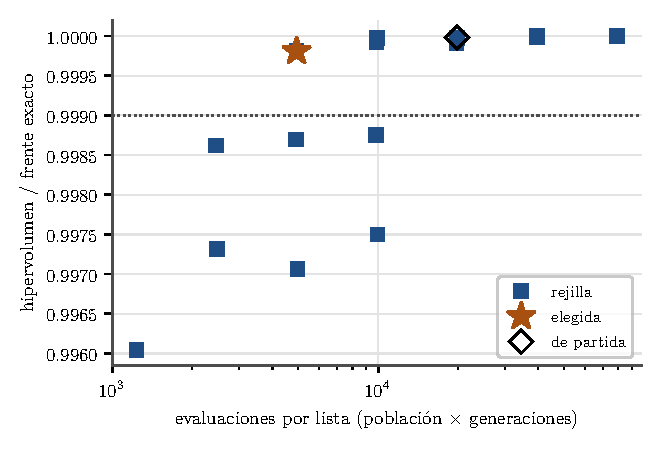
\includegraphics[width=\linewidth]{img/calibracion/rejilla.pdf}\end{minipage}\hfill
\begin{minipage}[t]{0.44\linewidth}\centering
{\footnotesize\textbf{(c)}}\\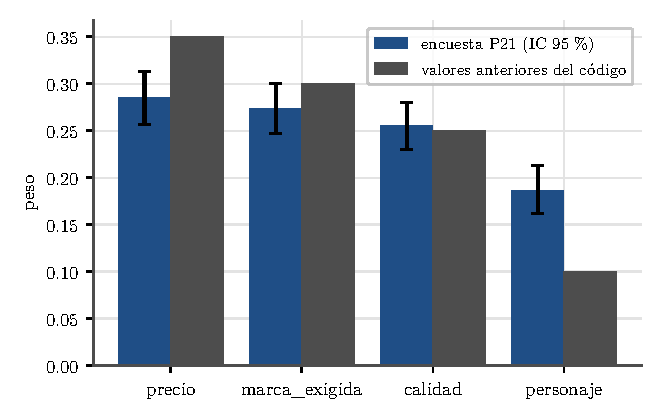
\includegraphics[width=\linewidth]{img/calibracion/pesos_p21.pdf}\end{minipage}\\[1mm]
\begin{minipage}[t]{0.44\linewidth}\centering
{\footnotesize\textbf{(d)}}\\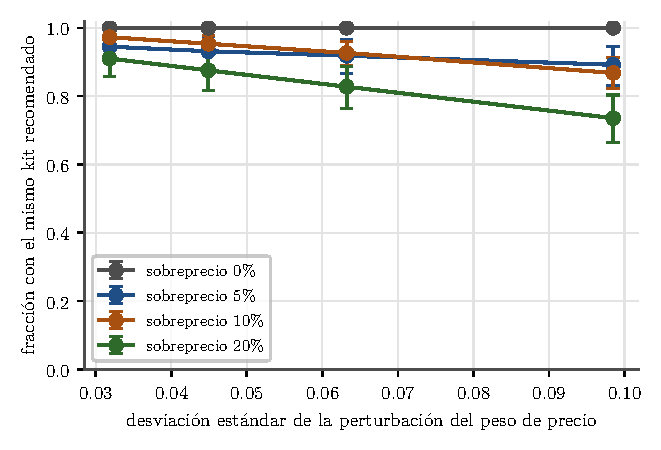
\includegraphics[width=\linewidth]{img/calibracion/sensibilidad.pdf}\end{minipage}\hfill
\begin{minipage}[t]{0.44\linewidth}\centering
{\footnotesize\textbf{(e)}}\\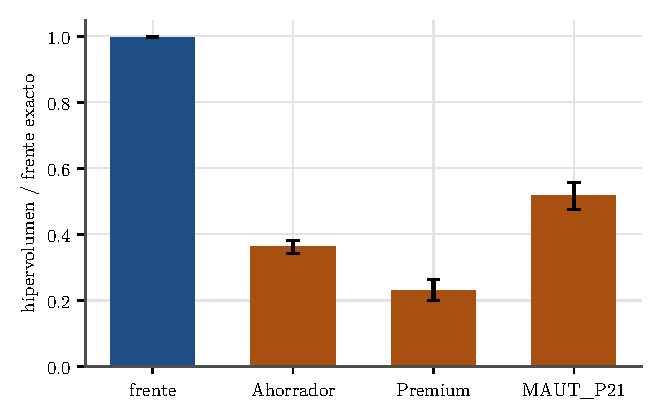
\includegraphics[width=\linewidth]{img/calibracion/hipervolumen_prueba.pdf}\end{minipage}
\caption[Gráficas de la calibración del optimizador.]{Calibración del optimizador. (a) Tiempo de la
enumeración exacta y de NSGA-II según el tamaño del espacio, y calidad del frente. (b) Rejilla de
población y generaciones. (c) Pesos de la P21 con su intervalo del 95\,\%. (d) Estabilidad del kit
recomendado bajo la perturbación de los pesos. (e) Hipervolumen relativo al frente exacto en las
listas de prueba.}
\label{fig:calibracion-graficas}
\end{figure}

Estos resultados tienen límites: los pesos salen de preferencias declaradas, la prueba tiene solo \calColegiosPrueba{} colegios, la calibración es retrospectiva y los tiempos son de una sola máquina; la Sección~\ref{sec:amenazas} los reúne con los del resto de la evidencia.
